\section{Hadoop Distributed File System}
\label{sec:hdfs}
\par HDFS pour \textit{Hadoop Distributed File System} est le système de fichiers propre à Hadoop. C'est le composant en charge du stockage des données dans un cluster Hadoop.

\subsection{Introduction}
\label{sec:introduction}

\par HDFS est un système de fichiers distribué, c'est-à-dire que contrairement à un système de fichiers local, il permet de stocker des fichiers de manière répartie sur plusieurs machines physiques. Du point de vue de l'utilisateur, l'ensemble des machines physiques n'est visible que sous la forme d'un espace de stockage géant. 

\begin{quote}
  \emph{A distributed system is a collection of independent computers that appear to the users of the system as a single computer.}
\end{quote}

\begin{flushright}
  Distributed Operating System. A. Tanenbaum, Prentice 
  Hall, 1994
\end{flushright}

\par Comparé aux autres systèmes de fichiers distribués, il partage beaucoup de points communs, mais présente toutefois des différences majeures, non négligeables.

\par HDFS est prévu pour du ``commodity hardware'', c'est-à-dire du matériel de grande distribution. Sa haute tolérance aux pannes lui permet de gérer du matériel ``low cost'', peu fiable, d'où sa popularité actuelle.

\par Pour finir cet aperçu, il est bon de noter que la réplication de données à travers les machines physiques rend l'accès aux données rapide, en plus de rendre le stockage résistant aux pannes.   

\subsection{Hypothèses de fonctionnement}
\label{sec:hypoth-de-fonct}

\subsubsection{Panne de matériel}
\label{sec:panne-de-materiel}

\par HDFS considère les pannes comme des événements qui peuvent se produire à tout moment. En effet, imaginons un cluster de mille noeuds ``low cost'', il paraît tout à fait concevable  qu'une machine tombe en panne (ou même plus). Cette supposition rend HDFS très résistant à ces pannes, et les mécanismes de réaction sont très rapides. La détection et l'adaptation rapides de ces pannes est un des principaux atouts de HDFS.

\subsubsection{Vitesse d'accès, gros volumes de données}
\label{sec:vitesse-dacces-aux}

\par Un système de fichiers classique est censé s'adapter à une utilisation moyenne. Ainsi, un exemple comme ext2 s'adapte à une taille de fichier moyenne inférieure à 3ko. Cela est un bon compromis en termes de rapidité d'accès moyenne et d'espace gaspillé par les clusters pas entièrement remplis. D'autre part, un ensemble de fonctionnalités permet de répondre à une demande hétérogène (POSIX).  Mais HDFS est prévu pour de grosses quantités de données (Big Data...), il serait ainsi ridicule de rechercher une grande performance de calcul, si elle est de toute façon limitée par la vitesse de lecture des données. C'est pour cela que HDFS déplace le compromis vers un point plus adapté, et permet ainsi une vitesse d'accès très élevée. Certaines fonctionnalités de systèmes de fichiers traditionnels ont été omises, du fait de leur inutilité pour ce cas d'utilisation précis, rendant HDFS encore plus performant dans son domaine.

\subsubsection{Modèle de cohérence simple}
\label{sec:modele-de-coherence}

\par Comme dit dans le paragraphe précédent, on recherche les cas d'utilisation de HDFS et on supprime toutes les fonctionnalités habituelles inutiles dans ce cas afin d'accéder à une plus grande performance. Une autre adaptation est donc celle du cycle de vie d'un fichier. Sur HDFS, on va créer un fichier (Write), puis y accéder massivement (Read), puis le fermer, mais on ne le modifiera jamais... Cette hypothèse simplifie beaucoup le problème de la cohérence des données, et rend l'accès encore plus rapide. Cela est donc particulièrement adapté aux applications MapReduce.
\par Un projet de fonctionnalité permettant d'ajouter des données en fin de fichier est en cours.

\subsubsection{``Moving Computation is Cheaper than Moving Data''}
\label{sec:moving-comp-cheap}

\par HDFS répond à un besoin classique du calcul distribué. Il s'agit simplement de dire qu'il est plus rapide d'effectuer un calcul sur les données là où elles sont stockées, et non de les déplacer. Cela permet de ne pas encombrer le réseau, et aussi de gagner en rapidité. HDFS met donc à disposition des interfaces pour déplacer les applications sur les noeuds qui contiennent les données (typiquement la fonction Map).

\subsubsection{Portabilité}
\label{sec:portabilite}

\par HDFS est prévu pour être installé sur une gamme très large de machines différentes

\subsection{Les démons HDFS}
\label{sec:demons_hdfs}

\par Le fonctionnement de HDFS est assuré par trois types de démons.

\subsubsection{Le NameNode}
\label{sec:namenode}

\par Le NameNode (NN) est un noeud maître disposant d'une machine dédiée. En effet, le NN est un \textit{SPOF} (\textit{Single Point Of Failure}). De ce fait, une panne du NN entraîne inéluctablement la panne de tout le cluster dans la mesure où seul le NN possède la cartographie des données. La seule façon de parer à une défaillance est de lui affecter une machine à haute tolérance aux pannes et d'avoir une machine \textquotedblleft{}mirroir\textquotedblright{} prête à démarrer en cas de défaillance.

\par Il héberge les métadonnées HDFS permettant ainsi de :

\smallskip

\begin{itemize}
\item réaliser la correspondance entre un fichier et les blocs le constituant;
\item localiser les blocs au sein du cluster, c'est-à-dire de faire la correspondance blocs/DataNode;
\item donner les informations relatives au propriétaire et autorisations des fichiers.
\end{itemize}

\smallskip

\par De ce fait, les métadonnées des blocs sont stockées sur disque dur (fichier \texttt{fsimage}) et chargées dans la mémoire vive du NN lors du démarrage du cluster. Les modifications intervenant dans le cluster sont répercutées immédiatement dans la mémoire vive du NN et enregistrées dans un journal (fichier \texttt{edits}) stocké sur disque dur.

\par La construction de la cartographie de la localisation des blocs dans le cluster est réalisée par les échanges d'informations qui ont lieu à chaque démarrage entre les DNs et le NN. Les DNs envoient ainsi au NN les métadonnées des blocs qu'ils contiennent.

\subsubsection{Le SecondaryNameNode}
\label{sec:secondarynamenode}

\par De la même manière, le SecondaryNameNode (SNN) est aussi un noeud maître disposant de sa propre machine dédiée. Contrairement à ce que l'on pourrait penser, le SNN n'est pas une copie de secours (\textit{backup}) du NN. Au contraire, il effectue les tâches de maintenance pour le compte du NN. Il consolide à intervalle régulier les modifications enregistrées dans le journal (fichier \texttt{edits}), et les reporte dans le fichier \texttt{fsimage} du NN. Ceci permet en outre de :

\begin{itemize}
\item garder sous contrôle l'espace disque utilisé par le journal;
\item limiter la charge processeur du NN;
\item réduire le temps de démarrage du NN, en limitant la taille du journal à \textquotedblleft{}rejouer\textquotedblright{} au démarrage.
\end{itemize}

\par Il intervient lorsque le fichier \texttt{edits} atteint une taille prédéfinie ou à intervalle régulier. Le paramétrage de ce dernier est laissé à l'utilisateur Hadoop.

\subsubsection{Le DataNode}
\label{sec:datanode}

\par Le DataNode (DN) est un noeud esclave implanté sur chaque machine du cluster. Dans celui-ci sont stockés les données des fichiers sous forme de blocs. Il peut contenir des blocs de différents fichiers.

\par Pour illustrer la répartition des démons au sein des machines, prenons pour exemple le cluster Skynet de Supélec qui contient 17 noeuds (\textit{sh00} à \textit{sh16}). Dans celui-ci vous trouverez trois noeuds maîtres correspondant au NameNode, SecondaryNameNode et JobTracker (Hadoop 1.x) ou ResourceManager (Hadoop 2.x). Il ne reste plus que 14 noeuds esclaves contenant chacun un DataNode et un TaskTracker (Hadoop 1.x) ou NodeManager (Hadoop 2.x).

\subsection{Lecture/Création d'un fichier HDFS par un programme Hadoop}
\label{sec:read-write-hdfs}

\par Afin de comprendre HDFS, il est essentiel de s'intéresser aux étapes mises en oeuvres afin de lire ou écrire un fichier sur HDFS. Pour information, les fonctions de gestion de fichiers sont issues du package Java \texttt{org.apache.hadoop}.

\paragraph{Lecture d'un fichier HDFS par un programme Hadoop (Figure~\ref{fig:lecture-hdfs}).}La demande d'ouverture du fichier HDFS par le programme Hadoop se fait via la fonction \texttt{open()}. HDFS se charge d'envoyer au NameNode la localisation des premiers blocs constituant le fichier par le biais d'un appel \textit{RPC} (\textit{Remote Procedure Call}). Le NameNode vérifie ensuite que le programme dispose des droits suffisants pour lire le fichier. Si les droits sont suffisants alors le NameNode renvoie à HDFS un nombre d'adresses pour chaque bloc correspondant au facteur de réplication des blocs, triées selon leur proximité par rapport à la JVM dans laquelle s'exécute le programme. En effet, au sein de chaque n\oe{}ud une JVM est lancée à l'exécution d'un job, chargée d'exécuter les ordres du TaskTracker (Hadoop 1.x) ou du NodeManager (Hadoop 2.x). 

\par Le programme accède ensuite au fichier en lecture via l'instruction \texttt{read()} après que HDFS lui ait renvoyé une instance du type \texttt{FSDataInputStream} afin d'établir la connexion avec le DataNode en question. Une fois la totalité du bloc lu, HDFS met fin à la connexion avec le DataNode concerné et en ouvre une nouvelle avec le bloc suivant. Il est important de remarquer que les blocs d'un même fichier peuvent se trouver sur des DataNodes différents.

\par En cas d'erreur de lecture, HDFS ferme la connexion avec le DataNode défaillant et en ouvre une autre avec le DataNode contenant le bloc le plus proche du dernier. Une fois que l'intégralité du fichier est lu, le programme Hadoop envoie l'instruction \texttt{close()} à l'instance \texttt{FSDataInputStream}, mettant ainsi fin à la lecture du fichier.

\begin{figure}[h!]
  \centering
  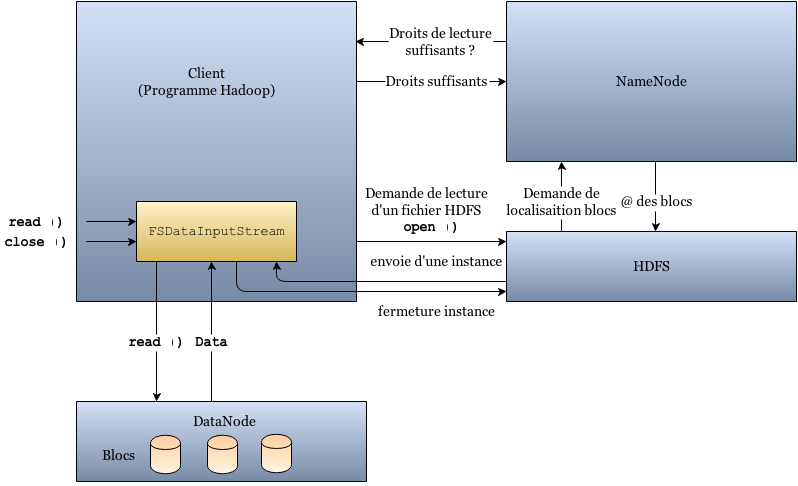
\includegraphics[width=16cm]{images/reading_file.png}
  \caption{Lecture d'un fichier HDFS par un programme Hadoop}
  \label{fig:lecture-hdfs}
\end{figure}

\paragraph{Création d'un fichier HDFS par un programme Hadoop (Figure~\ref{fig:ecriture-hdfs}).} Lors de la création d'un fichier, le programme Hadoop fait une demande à HDFS par le biais de l'instruction \texttt{create()}. HDFS transmet la demande de création au NameNode avec un appel de type \textit{RPC}. Ce dernier s'assure que le fichier n'a pas déjà été créé et que le programme dispose des droits suffisants pour sa création. Si tel est le cas, le NameNode intègre le nouveau fichier dans sa cartographie des données du cluster et tout comme dans le cas d'une lecture, HDFS envoie une instance de type \texttt{FSDataOutputStream} au programme, ce qui lui permet d'accéder au fichier en écriture.

\par Les modifications en écriture du fichier sont envoyés à HDFS sous forme de paquets (\textit{packets}) et stockés temporairement dans une file d'attente (\textit{data queue}), prise en charge par une instance \texttt{DataStreamer}. Cette dernière demande au NameNode les adresses de deux blocs (égal au nombre de réplication) sur deux DataNodes différents afin d'y stocker les données en file d'attente. Un accusé de réception du paquet (\textit{packet acknowledged}) stocké avec succès est envoyé à l'instance \texttt{FSDataOutputStream}. A la fin de cette opération, l'instance \texttt{DataStreamer} demande à nouveau deux nouvelles adresses au NameNode. L'opération se répète jusqu'à ce que tous les blocs d'un même fichier aient été stockés convenablement.

\par En cas d'erreur d'écriture au niveau d'un DataNode, HDFS est en mesure de détecter cela car un accusé de réception pour un certain paquet ne lui sera pas parvenu. Pour pallier à ce problème, HDFS dispose de mécanismes permettat de rétablir une situation normale, via l'affection d'un bloc de remplacement dans le cluster et la réécriture de tous les paquets susceptibles d'être affectés par le problème d'écriture dans ce nouveau bloc.

\par Enfin, lorsque le dernier paquet est écrit avec succès sur les deux DataNodes différents, le programme Hadoop envoie l'instruction \texttt{close()} à l'instance \texttt{FSDataOutputStream}.

\begin{figure}[h!]
  \centering
  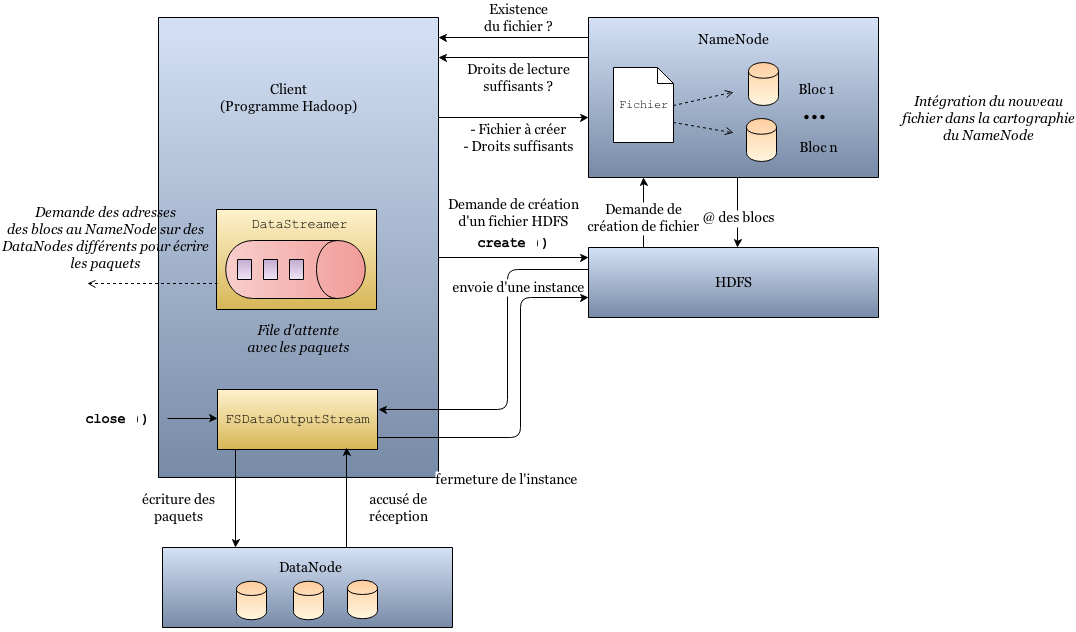
\includegraphics[width=17cm]{images/writing_file.png}
  \caption{\'{E}criture d'un fichier HDFS par un programme Hadoop}
  \label{fig:ecriture-hdfs}
\end{figure}

\paragraph{Vue d'ensemble (Figure~\ref{fig:archi-hdfs}).} Ci-dessous est donnée la vue d'ensemble de l'architecture du système de fichiers de Hadoop. On y retrouve les opérations de lecture et écriture explicitées précédemment. Le NameNode se trouve au c\oe{}ur de cette architecture : c'est lui qui gère l'ensemble des métadonnées des blocs contenus dans les DataNodes.

\par Cette vue met en lumière un autre aspect de Hadoop. Au sein de très gros clusters, il est possible d'adopter une organisation des machines par \textit{racks}. Pour plus de sécurité, Hadoop tâchera de répliquer les données dans des \textit{racks} différents. En effet, la politique de tolérance zéro aux pannes implique que, dans le cas d'un \textit{rack} défaillant, il soit possible de récupérer les données dans un autre \textit{rack}. De cette façon, Hadoop évite de perdre des données en cas de panne.

\begin{figure}[ht!]
  \centering
  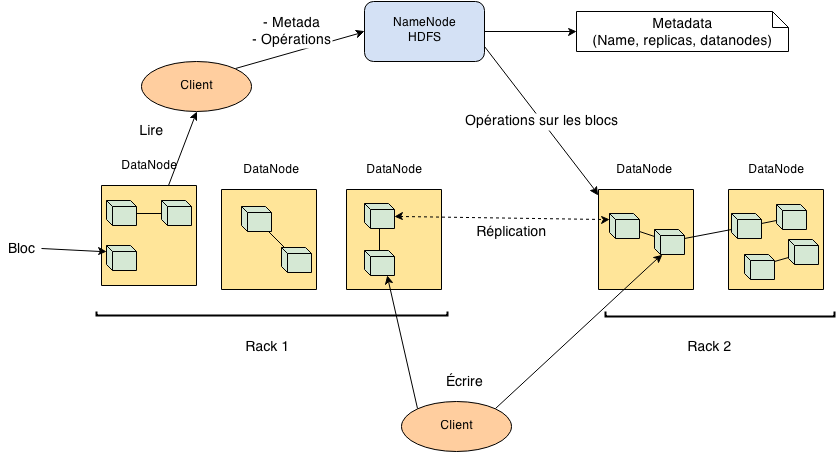
\includegraphics[width=16cm]{images/hadoop_arch.png}
  \caption{Architecture HDFS}
  \label{fig:archi-hdfs}
\end{figure}

%%% Local Variables:
%%% mode: latex
%%% TeX-master: "CompteRendu"
%%% End: 
